\documentclass[a4paper]{report}
% Shared preamble for the English probability and statistics documents.
% Based on the original course preamble. Compile with pdfLaTeX.
\usepackage[top=1.5cm,bottom=2cm,left=2cm,right=2cm]{geometry}
\usepackage[T1]{fontenc}
\usepackage{lmodern}
\usepackage[utf8]{inputenc}
\usepackage[english]{babel}

\usepackage{amsmath}
\usepackage{amssymb}
\usepackage{amsthm}
\usepackage{mathrsfs}
\usepackage{mathtools}
\usepackage{etoolbox}
\usepackage{tikz}
\usetikzlibrary{shapes.multipart,arrows.meta}
\usepackage{xcolor}
\usepackage{enumerate}
\usepackage[shortlabels]{enumitem}
\usepackage{hyperref}
\usepackage{version}
\usepackage{bbold}
\usepackage{fontawesome5}
\usepackage{fancyhdr}
\lfoot{}
\usepackage{natbib}
\usepackage{graphicx}
\usepackage{pdfpages}
\usepackage{authblk}
    
\usepackage{blindtext}
\usepackage{multicol}
\usepackage{collcell}
\usepackage{wrapfig}
\usepackage{blkarray}
\usepackage{cancel}
\usepackage{appendix}
\usepackage{float}
\makeatletter
\input{tex/assets/slashbox.sty}
\makeatother
\hypersetup{unicode,colorlinks,citecolor=red,filecolor=black,
  linkcolor=red,urlcolor=cyan}
\setlength{\columnsep}{1cm}
\pagenumbering{gobble}

\def\numtext#1{%
  \ifcase#1\or one\or two\or three\or four\or five\or six\or seven\or eight\or nine\or ten\or
  eleven\or twelve\or thirteen\or fourteen\or fifteen\or sixteen\or seventeen\or eighteen\or nineteen\or twenty\or Lots\fi}

\newcommand{\Byte}[1]{%
  \def\nodecontents{}%
  \foreach[count=\l] \k in {#1} {\xappto{\nodecontents}{\noexpand\nodepart{\numtext{\l}}\k}}%
  \node[rectangle split,rectangle split parts=8,rectangle split horizontal,draw] at (2,2){\nodecontents};}

\newcommand{\D}{{\mathrm{d}}}
\newcommand{\cE}{{\mathcal{E}}}
\newcommand{\cG}{{\mathcal{G}}}
\newcommand{\cX}{{\mathcal{X}}}
\newcommand{\cY}{{\mathcal{Y}}}
\newcommand{\cB}{{\mathcal{B}}}
\newcommand{\cF}{{\mathcal{F}}}
\newcommand{\cO}{{\mathcal{O}}}
\newcommand{\cS}{{\mathcal{S}}}
\newcommand{\cT}{{\mathcal{T}}}
\newcommand{\given}{\, \big| \,}
\newcommand{\cL}{{\mathscr{L}}}
\newcommand{\cD}{{\mathcal{D}}}
\newcommand{\cA}{{\mathscr{A}}}
\newcommand{\cP}{{\mathscr{P}}}
\newcommand{\cR}{{\mathscr{R}}}
\newcommand{\A}{{\mathcal A}}
\newcommand{\one}{\mathbb{1}}
\newcommand{\mathbbm}[1]{\mathbb{#1}}

\providecommand{\C}{}
\renewcommand{\C}{\mathbb C}
\newcommand{\R}{\mathbb R}
\newcommand{\Q}{\mathbb Q}
\newcommand{\N}{\mathbb N}
\newcommand{\T}{\mathbb T}
\newcommand{\F}{\mathbb F}
\renewcommand{\P}{\mathbb P}
\newcommand{\Z}{\mathbb Z}
\newcommand{\E}{\mathbb {E}}
\newcommand{\Pbb}[1]{\P\left( #1\right)}
\newcommand{\Ebb}[1]{\E\left[ #1\right]}

\newcommand{\lb}{\left (}
\newcommand{\rb}{\right )}
\newcommand{\lbb}{\left [}
\newcommand{\rbb}{\right ]}
\newcommand{\labs}{\left |}
\newcommand{\rabs}{\right |}
\newcommand{\lbrb}[1]{\lb #1 \rb}
\newcommand{\lbbrbb}[1]{\lbb#1\rbb}
\newcommand{\labsrabs}[1]{\labs#1\rabs}
\newcommand{\lbbrb}[1]{\lbb#1\rb}
\newcommand{\lbrbb}[1]{\lb#1\rbb}
\newcommand{\langlerangle}[1]{\langle#1\rangle}
\newcommand{\lbcurly}{\{}
\newcommand{\rbcurly}{\}}
\newcommand{\curly}[1]{\lbcurly#1\rbcurly}
\newcommand{\abs}{\labsrabs}
\newcommand{\ind}[1]{1_{#1}}
\newcommand{\indep}{\perp \!\!\! \perp}
\renewcommand{\d}{\, \mathrm{d}}

\newtheorem{theorem}{Theorem}
\newtheorem{problemCnt}{Lemma}
\theoremstyle{definition}
\newtheorem{problem}[problemCnt]{Problem}
\newtheorem{problembook}[problemCnt]{\faBook \,  Problem}
\newtheorem{problempencil}[problemCnt]{\faPencil* \,  Problem}
\newtheorem{problemstar}[problemCnt]{\faStar\,  Problem}
\newtheorem{problemstarpencil}[problemCnt]{\faStar \, \faPencil* \,   Problem}
\newtheorem{probleminteresting}[problemCnt]{\faSmile[regular] \,   Problem}
\newtheorem{solution}{Solution}

\newcommand{\fwcell}[1]{\makebox[\arraystretch\normalbaselineskip]{$#1$}}
\newenvironment{enumeratei}{\begin{enumerate}[(i)]}{\end{enumerate}}
\newenvironment{enumeratea}{\begin{enumerate}[(a)]}{\end{enumerate}}
\newenvironment{enumeraten}{\begin{enumerate}[\upshape 1.]}{\end{enumerate}}

% Compatibility helpers needed by a few files in the combined archive.
\AtBeginDocument{\noindent{\footnotesize English translation prepared with ChatGPT (OpenAI, GPT-6), 26 October 2026, for translation of the Bulgarian text into English and LaTeX formatting.
The Bulgarian originals remain the reference; translation may contain errors.}\par\smallskip}
\newcommand{\MissingGraphic}[1]{%
  \begin{center}\fbox{\parbox{0.82\linewidth}{\centering Missing source image: \texttt{#1}}}\end{center}}



\setlength{\emergencystretch}{3em}
\allowdisplaybreaks
\begin{document}


\noindent Probability and Statistics \hfill Written exam, 01.02.2023

\hrulefill

\begin{it}
The exact grading formula depends on the results.
The minimum score required
to pass is 1 point. As an approximation, use 2 plus the points earned. Time allowed: 3 hours. Good luck.

Integration formulas:
$\int u \, \mathrm{d} v = uv - \int
v \, \mathrm{d} u$, $\mathrm{d} f(x) =
f'(x) \mathrm{d} x$.
\end{it}

\begin{problem}
A standard roulette wheel has 18 red, 18
black and one green number. For a successful
bet on
black/red, the casino pays
twice the stake.

\begin{enumerate}
    \item (0.5 points) Assume all bets are BGN 1. How many bets per day must the casino accept so that its profit is at least
    BGN 1000 with probability 90\%?
    With this many bets, what is the probability that the casino makes a loss
    on a given day?
    \item (0.25 points) One may also bet on a single number, with a payout of
    36 times the stake. Which would you prefer: betting on one number or on black/red? (Compare
    the expectations and variances and make your choice
    using them.)

    \item (0.25 points) If you have BGN 5, which would you prefer:
    five bets on a number over
    five spins, bets on five different numbers in one spin, or a BGN 5 bet on black/red in one spin?




\end{enumerate}

\end{problem}

\begin{problem}
Let the joint density of $X$ and $Y$ be $f_{X,Y}(x,y)=cx^3y$ for $x,y\geq0$, $x+y\leq1$, and zero elsewhere, where $c$ is
a constant. Find:

\begin{enumerate}

    \item (0.5 points) $c$, the density of $X$ and the expectation of $Y$.
    Explain how you would calculate
     $Cor(X, Y)$;
\item (0.25 points) $\E(Y|X=1/2)$ and
$\E(X|X=1/2)$;
\item (0.25 points) the density of the random variable $Z=XY$.

\end{enumerate}
\end{problem}


\begin{problem}

The cells of a $9\times9$ grid are
coloured at random in one of the colours
white, green and red.

\[ 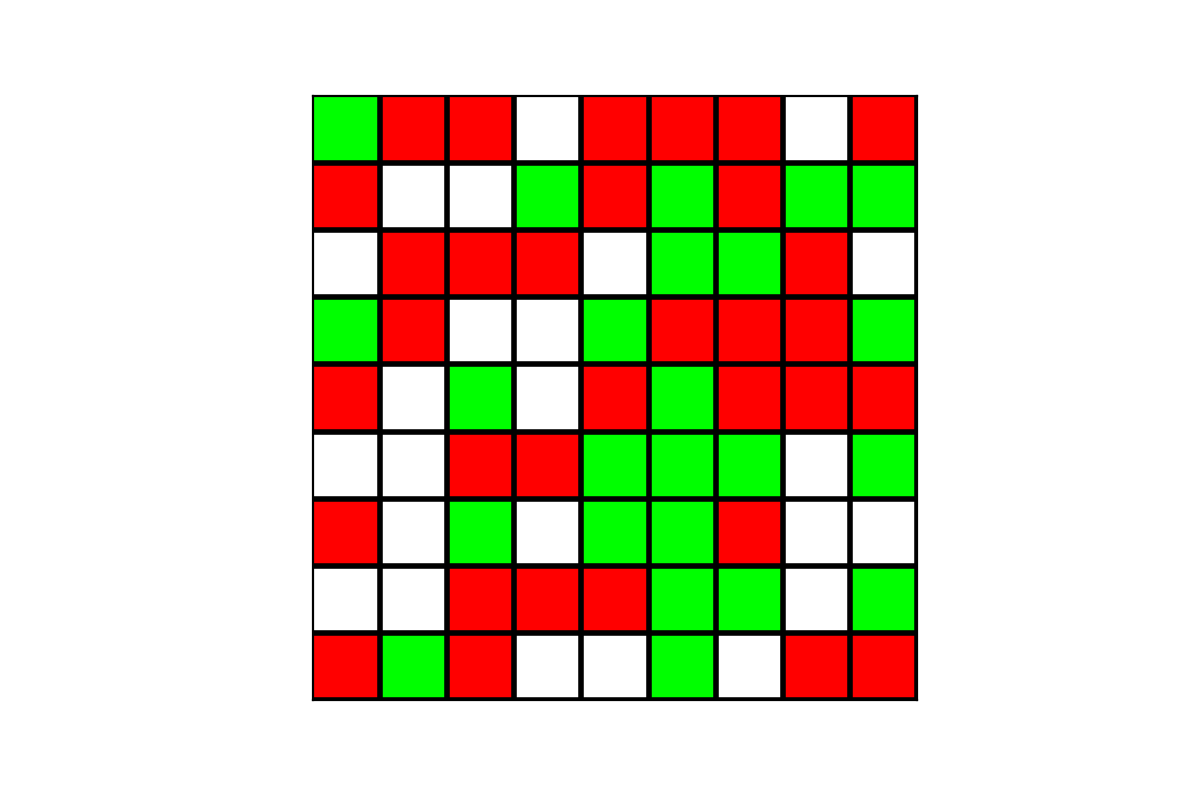
\includegraphics[width=0.4\textwidth]{tex/assets/prob-stat/grid.png}
 \]




\begin{enumerate}
    \item (0.5 points) What is the expected number of cells coloured
    white or green?
    What is the probability that there are at least 60 such cells?

    A horizontal (vertical) flag is
    three consecutive horizontal (vertical) cells coloured
    white, green and red from left
    to right (top to bottom).

    \item (0.25 points)
    Is the number of horizontal
    flags binomially distributed?
    If so, what are its parameters?
    \item (0.25 points)
    What is the expected number of horizontal
    flags?
    \item (0.25 points)
    Are the numbers of horizontal
    and vertical flags independent?
    What is the expected total number of
    horizontal AND vertical
    flags?
\end{enumerate}
\end{problem}


\begin{problem}
    Let $X_1,X_2,\dots$ be independent
    $Exp(1)$ random variables and
    $S_n = X_1 + \dots + X_n$.

    \begin{enumerate}
        \item (0.5 points) Find the density
        of $S_2$ and prove by induction
        that the density of $S_n$ is
        \[
        f_{S_n}(x) = \frac{x^{n-1}}{(n-1)!}{e^{-x}}\one_{\{x>0\}}.
        \]
        \item (0.25 points)
        Let $N_t:=\max\{n:S_n\leq t\}$.
        Prove that $\P(N_t\geq n)
        =\P(S_n\leq t)$ and that
        $\P(N_t = n) =
        \P(S_n \leq t) - \P(S_{n+1} \leq t)$.
        \item (0.25 points)
        Find the distribution of
        $N_t$.
    \end{enumerate}


\end{problem}















































\end{document}
